\documentclass{article}
\usepackage{tikz}

\begin{document}
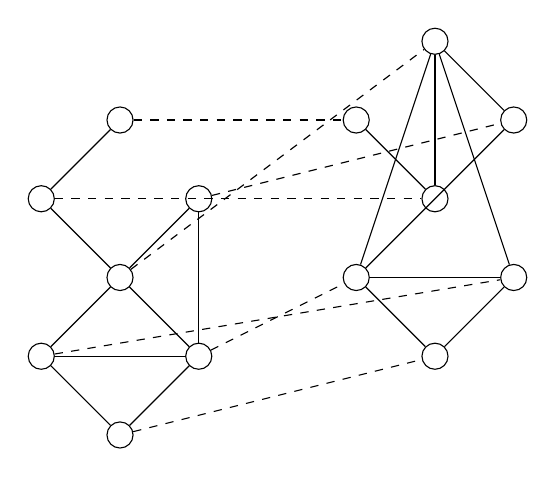
\begin{tikzpicture}
    % Graph 1 nodes
    \path
    (1, 0) node[circle, draw] (A1) {}
    (0, 1) node[circle, draw] (B1) {}
    (2, 1) node[circle, draw] (C1) {}
    (1, 2) node[circle, draw] (D1) {}
    (0, 3) node[circle, draw] (E1) {}
    (2, 3) node[circle, draw] (F1) {}
    (1, 4) node[circle, draw] (G1) {}
    ;

    % Graph 1 edges
    \draw (A1) -- (B1);
    \draw (A1) -- (C1);
    \draw (B1) -- (C1);
    \draw (B1) -- (D1);
    \draw (C1) -- (D1);
    \draw (C1) -- (F1);
    \draw (D1) -- (E1);
    \draw (D1) -- (F1);
    \draw (E1) -- (G1);

    % Graph 2 nodes (rotated)
    \path
    (5, 1) node[circle, draw] (A2) {}
    (6, 2) node[circle, draw] (B2) {}
    (4, 2) node[circle, draw] (C2) {}
    (5, 5) node[circle, draw] (D2) {}
    (5, 3) node[circle, draw] (E2) {}
    (6, 4) node[circle, draw] (F2) {}
    (4, 4) node[circle, draw] (G2) {}
    ;

    % Graph 2 edges
    \draw (A2) -- (B2);
    \draw (A2) -- (C2);
    \draw (B2) -- (C2);
    \draw (B2) -- (D2);
    \draw (C2) -- (D2);
    \draw (C2) -- (F2);
    \draw (D2) -- (E2);
    \draw (D2) -- (F2);
    \draw (E2) -- (G2);

    % Matching edges
    \draw[dashed] (A1) -- (A2);
    \draw[dashed] (B1) -- (B2);
    \draw[dashed] (C1) -- (C2);
    \draw[dashed] (D1) -- (D2);
    \draw[dashed] (E1) -- (E2);
    \draw[dashed] (F1) -- (F2);
    \draw[dashed] (G1) -- (G2);

\end{tikzpicture}
\end{document}
